\section{Umsetzung}\label{sec:umsetzung}

\subsection{Resultate}

\subsubsection{Zusammenfassung}

Das Praxisrufsystem wurde wie im Kapitel Konzept beschrieben umgesetzt.
Es wurden die drei Komponenten Mobile Client, Cloud Service und Admin UI implementiert.
Über den angebundenen Messaging Service Firebase Messaging ist es möglich, Benachrichtigungen zwischen Mobile Clients zu versenden.
Cloud Service und Admin UI ermöglichen es dabei die Benachrichtigungen die Versendet werden können und welcher Client welche Benachrichtungen erhalten soll zu konfigurieren.
Weiter wurde mit Amazon Web Services (AWS) eine CI/CD Umgebung aufgebaut, die es erlaubt Cloud Service und das Admin UI zu betreiben und testen.
Diese Umgebung wird dem Kunden als Template dienen, wie er das Praxisrufsystem in der Praxis betreiben kann.
Detaillierte Informationen dazu finden sich im Betriebshandbuch im Anhang.


\subsubsection{Umgesetzte Anforderungen}

Im Rahmen des Projektes konnten die folgenden User Stories inklusive aller dazu definierten Features und Szenarien umgesetzt werden:

\begin{itemize}
    \item U01: Benachrichtigungen versenden können.
    \item U02: Als Praxismitarbeiter möchte ich Benachrichtigungen empfangen können, damit ich auf Probleme und Anfragen anderer Mitarbeiter reagieren kann.
    \item U03: Als Praxismitarbeiter möchte ich nur Benachrichtigungen sehen, die für mich relevant sind, damit ich meine Arbeit effizient gestalten kann.
    \item U04: Als Praxismitarbeiter möchte ich über empfangene Benachrichtigungen aufmerksam gemacht werden, damit ich keine Benachrichtigungen verpasse.
    \item U05: Als Praxismitarbeiter möchte ich sehen welche Benachrichtigungen ich verpasst habe, damit ich auf verpasste Benachrichtigungen reagieren kann.
    \item U06: Als Praxismitarbeiter möchte ich eine Rückmeldung erhalten, wenn eine Benachrichtigung nicht versendet werden kann, damit Benachrichtigungen nicht verloren gehen.
    \item U07: Als Praxismitarbeiter möchte ich auswählen können an welchem Gerät ich das Praxisrufsystem verwende und die dafür erstellte Konfiguration erhalten, damit das Praxisrufsystem optimal verwendet werden kann.
    \item U12: Als Praxisverantwortlicher möchte ich mehrere Geräte verwalten können, damit das Praxisrufsystem in mehreren Zimmern gleichzeitig genutzt werden kann.
    \item U13: Als Praxisverantwortlicher möchte ich definieren können welches Gerät, welche Anfragen versenden kann, damit jedes Gerät Verwendungsort optimiert ist.
    \item U14: Als Praxisverantwortlicher möchte ich die Konfiguration des Praxisrufsystems zentral verwalten können, damit das Praxisrufsystem für die Anwender optimiert werden kann.
    \item T01: Als Auftraggeber möchte ich, dass das Praxisrufsystem über IPads bedient werden kann, damit ich von bestehender Infrastruktur profitieren kann.
    \item T02: Als Auftraggeber möchte ich, dass das Praxisrufsystem über Android Tablets bedient werden kann, damit es in Zukunft für eine weitere Zielgruppe verwendet werden kann.
    \item T03: Als Auftraggeber möchte ich, dass die Codebasis für das Praxisrufsystem für Android und IOS verwendet werden kann, damit ich die Weiterentwicklung optimieren kann.
    \item T04: Als Auftraggeber möchte ich, dass wo möglich der Betrieb von Serverseitigen Dienstleistungen über AWS betrieben wird, damit ich von bestehender Infrastruktur und Erfahrung profitieren kann.
\end{itemize}

\subsubsection{Abgrenzung}

Die folgenden User Stories konnten im Rahmen des Projektes nicht realisiert werden:

\begin{itemize}
    \item U08: Als Praxismitarbeiter möchte ich einen physischen Knopf am Behandlungsstuhl haben damit ich notifikationen darüber versenden kann.
    \item U09: Als Praxismitarbeiter möchte ich, dass mir Benachrichtigungen vorgelesen werden, damit ich informiert werde, ohne meine Arbeit unterbrechen zu müssen.
    \item U10: Als Praxismitarbeiter möchte ich einen anderen Client Unterhaltungen führen können damit Fragen direkt geklärt werden können.
    \item U11: Als Praxismitarbeiter möchte ich Unterhaltungen mit mehreren anderen Clients gleichzeitig führen können damit komplexe Fragen direkt geklärt werden können.
    \item U15: Als Praxisverantwortlicher möchte ich definieren können, welche Geräte mit welchen anderen Geräten telefonieren können damit meinen Mitarbeitern das Arbeiten erleichtere.
    \item U16: Als Praxisverantwortlicher möchte ich definieren können, welche Benachrichtigung über einen physischen Knopf am Behandlungsstuhl versendet wird damit der Knopf für den Mitarbeiter optimiert ist.
\end{itemize}


Abweichungen vom Konzept
\begin{itemize}
    \item Die Gegensprechanlage ist komplett Weggefallen.
    \subitem Grundsätzlich Stünde eine Lib. für IOS in NS zur Verfügung. Der Android Teil ist da noch "TODO"
    \item Die Rückfärbung der Buttons auf Grün ist weggefallen da der Handshake so nicht implmentiert wurde.
\end{itemize}

\clearpage
\subsubsection{Mobile Client}\label{subsec:mobile-client-realisation}

Dieses Kapitel zeigt die umgesetzten Ansichten des Mobile Clients.
Eine detaillierte Beschreibung, wie der Mobile Client bedient werden kann, befindet sich im Anhang der Projektdokumentation.

\begin{figure}[h]
    \centering
    \begin{minipage}[b]{0.4\textwidth}
        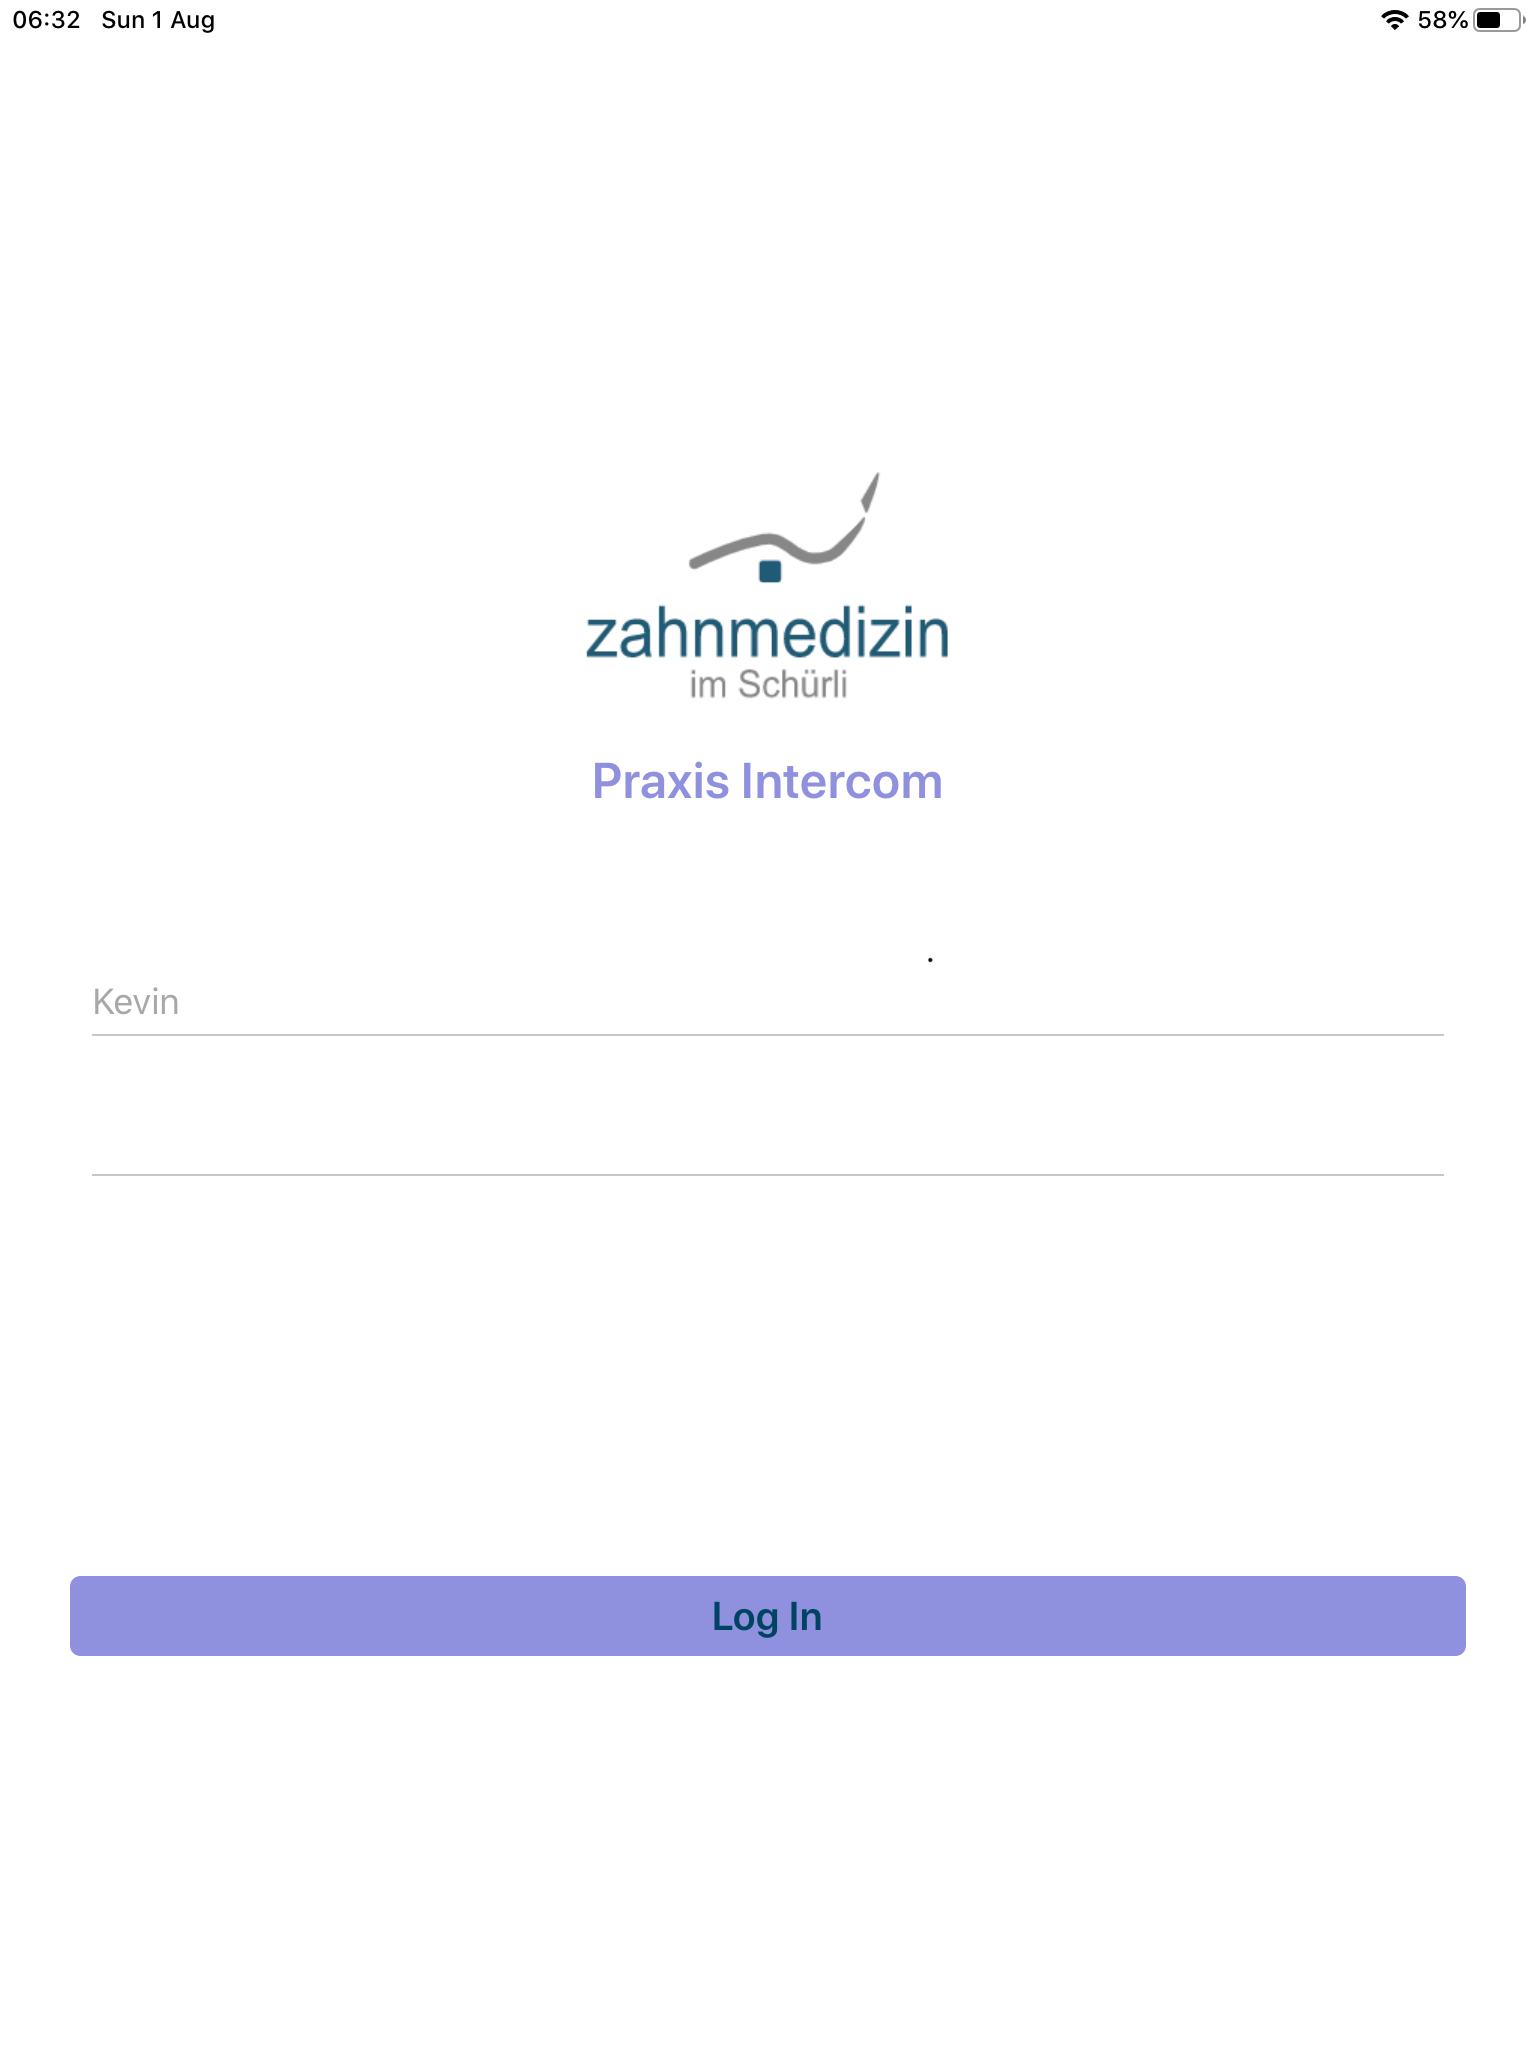
\includegraphics[width=\textwidth]{graphics/screenshot-login}
        \caption{Login}
    \end{minipage}
    \hfill
    \begin{minipage}[b]{0.4\textwidth}
        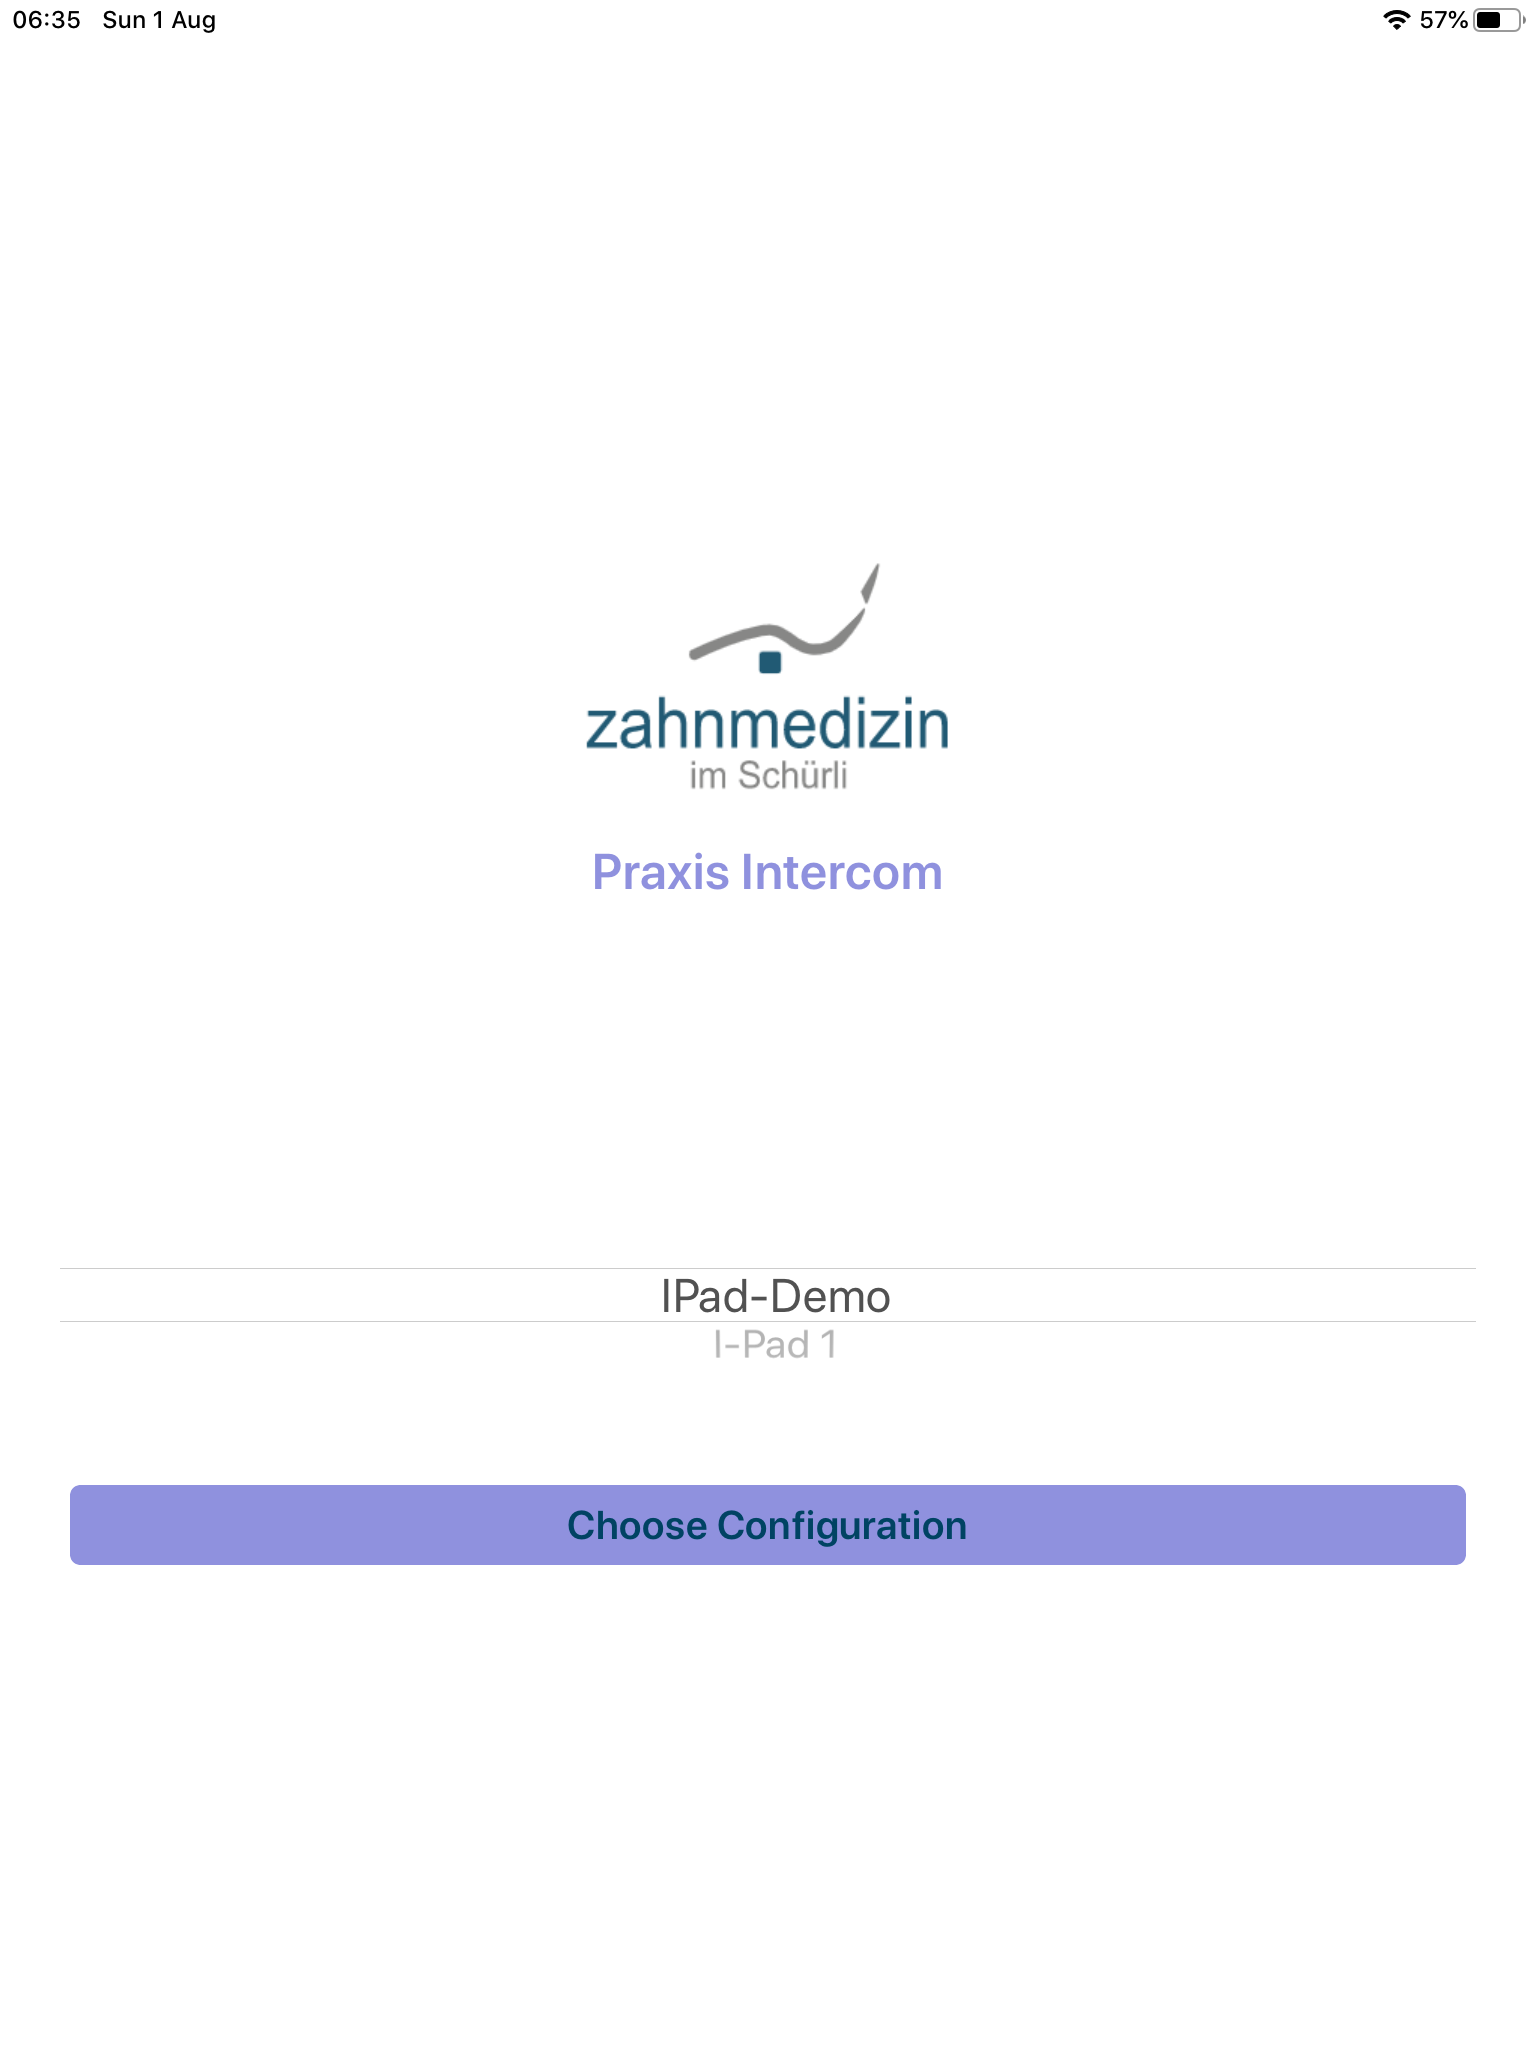
\includegraphics[width=\textwidth]{graphics/screenshots/mobileclient/screenshot-select-config}
        \caption{Konfiguration}
    \end{minipage}
    \label{fig:MobileClient-Screens1}
\end{figure}

\clearpage

Dieses Kapitel zeigt die umgesetzten Ansichten des Admin UIs.
Eine detaillierte Beschreibung, wie der Mobile Client bedient werden kann, befindet sich im Anhang der Projektdokumentation.

\begin{figure}[h]
    \centering
    \begin{minipage}[b]{0.4\textwidth}
        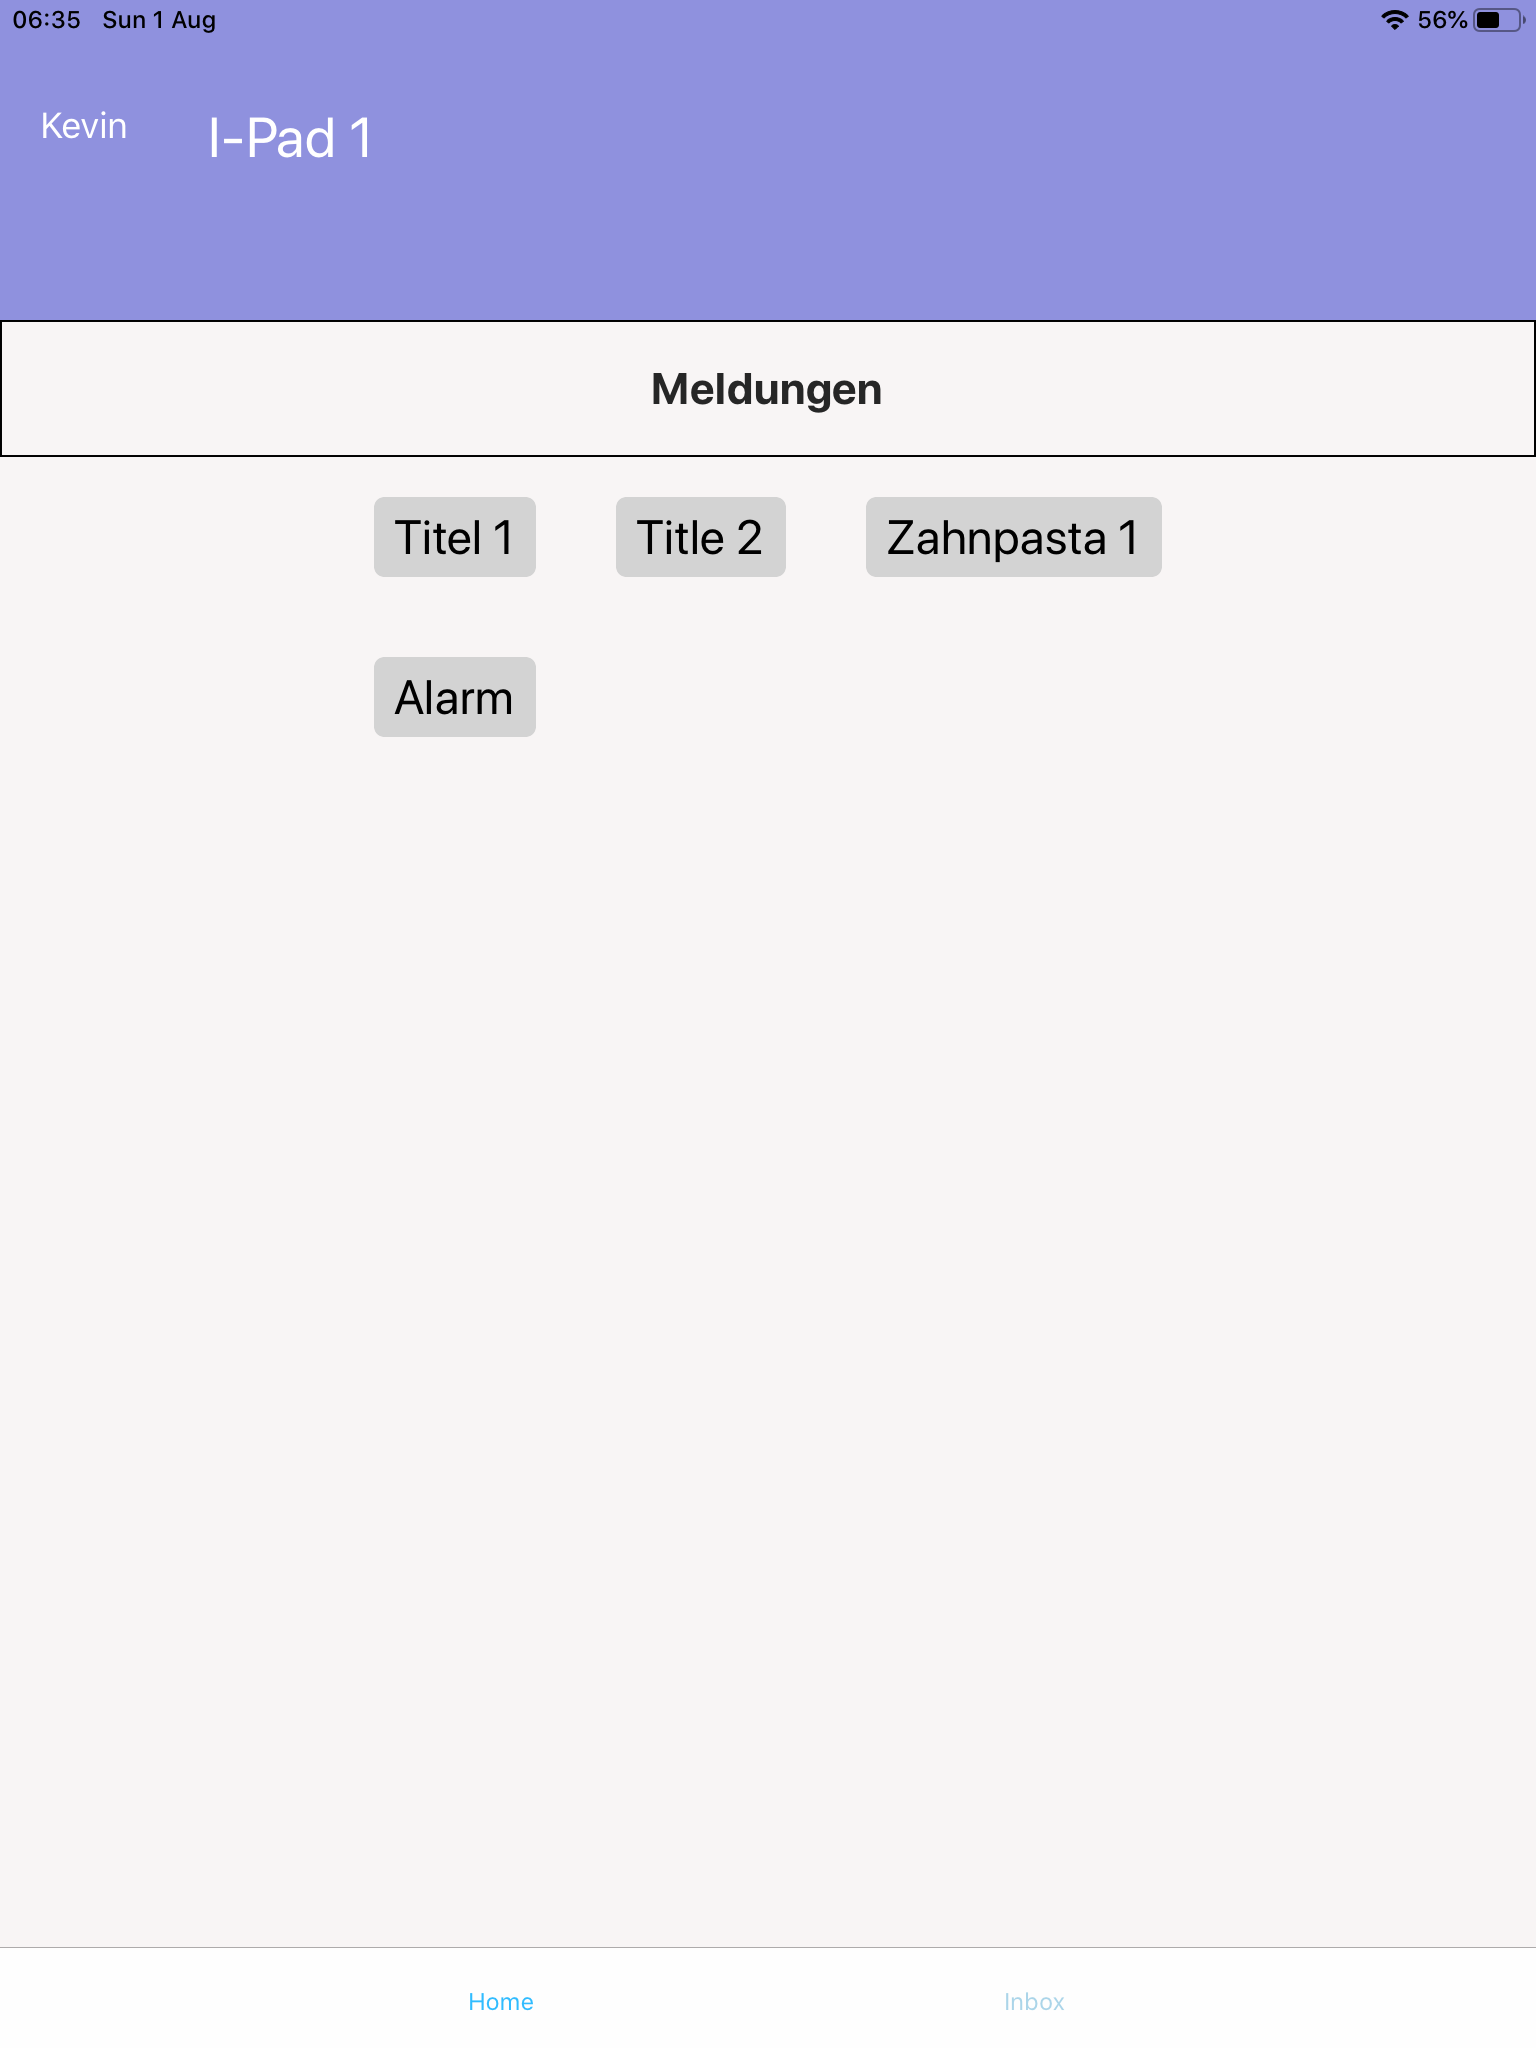
\includegraphics[width=\textwidth]{graphics/screenshots/mobileclient/screenshot-homescreen}
        \caption{Home}
    \end{minipage}
    \hfill
    \begin{minipage}[b]{0.4\textwidth}
        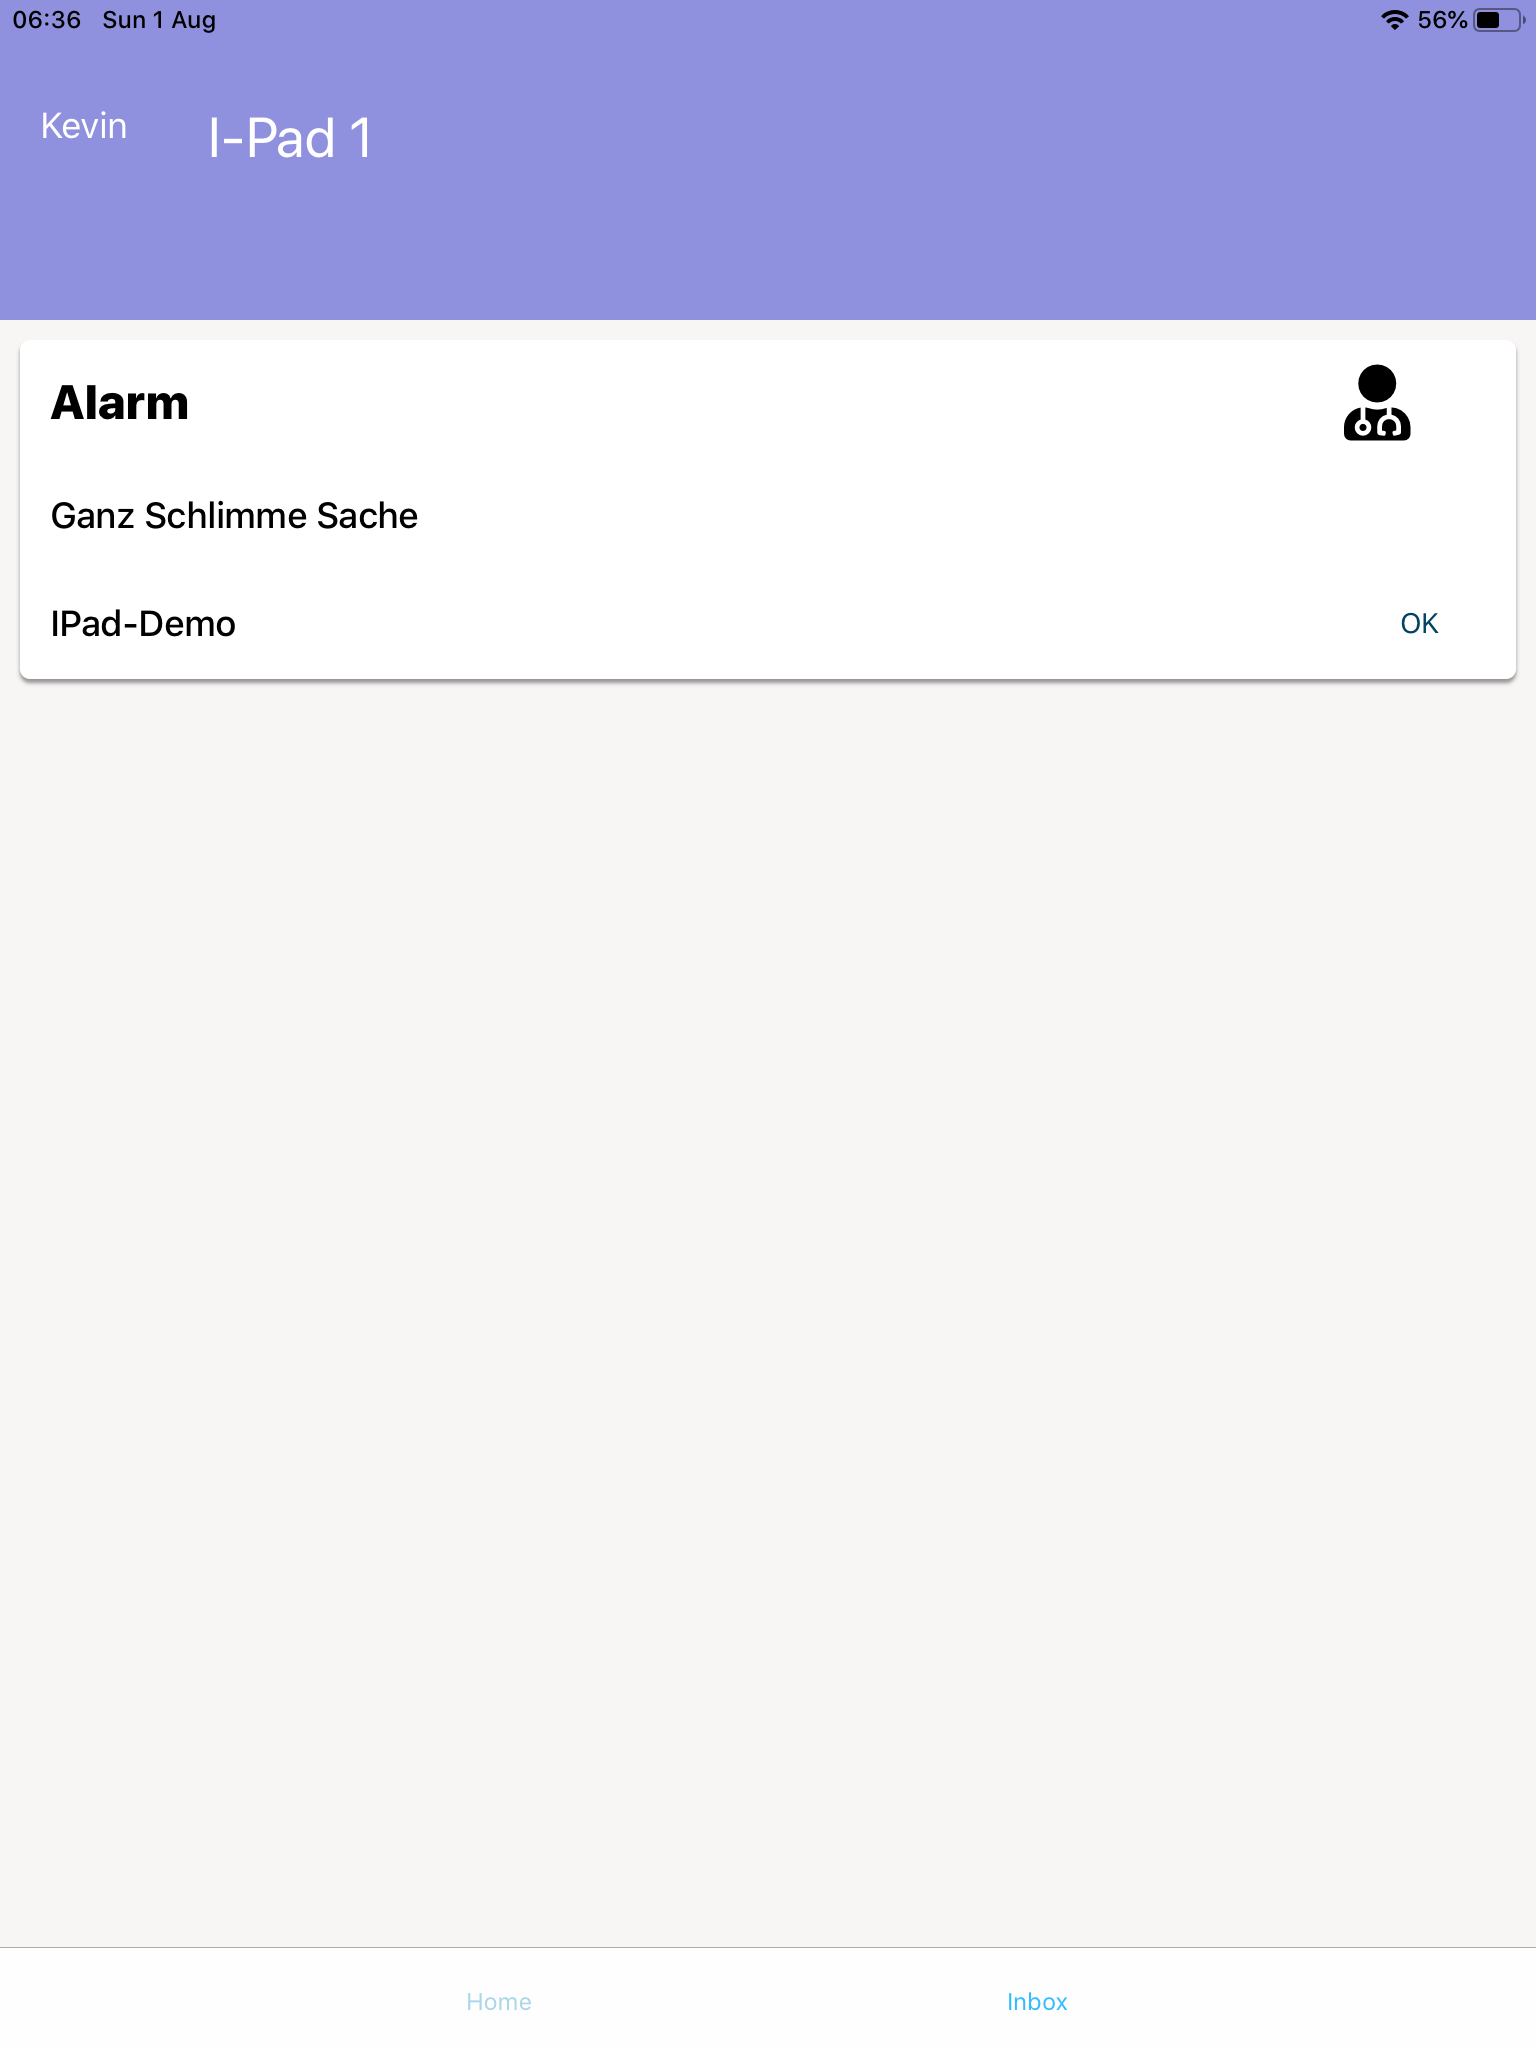
\includegraphics[width=\textwidth]{graphics/screenshots/mobileclient/screenshots-inbox}
        \caption{Inbox}
    \end{minipage}
    \label{fig:MobileClient-Screens2}
\end{figure}

\clearpage

\subsubsection{Cloud Service}

Der Cloud Service wurde wie im Konzept beschrieben umgesetzt und an den Messaging Service angebunden.

Die API ist unter www.praxisruf.ch/api erreichbar.
www.praxisruf.ch/swagger-ui.html bietet zudem zu Testzwecken die Möglichkei die Endpoints direkt anzusprechen.

\begin{minipage}[b]{1\textwidth}
    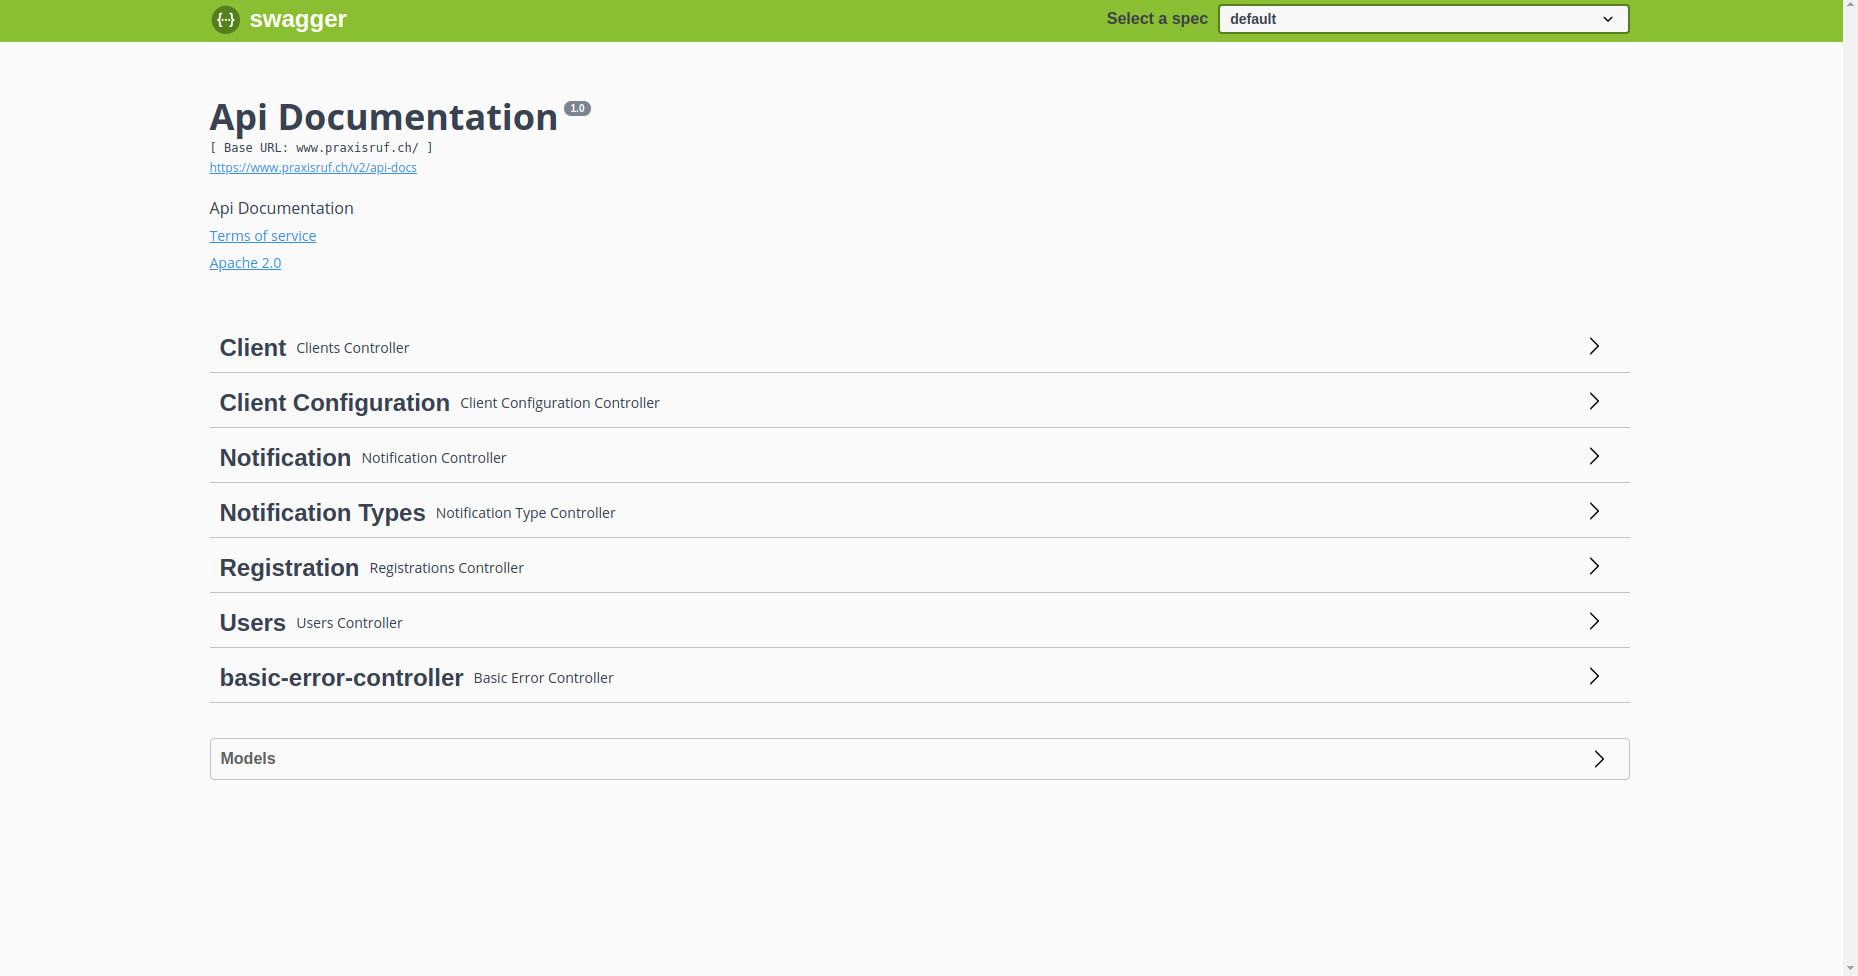
\includegraphics[width=\textwidth]{graphics/screenshots/cloud/swagger-home}
    \caption{Home}
\end{minipage}

Sorgt neben der API auch die Authentifikation die umgesetzt wurde.

\clearpage

\subsubsection{Admin UI}

\begin{figure}[h]
    \centering
    \begin{minipage}[b]{0.4\textwidth}
        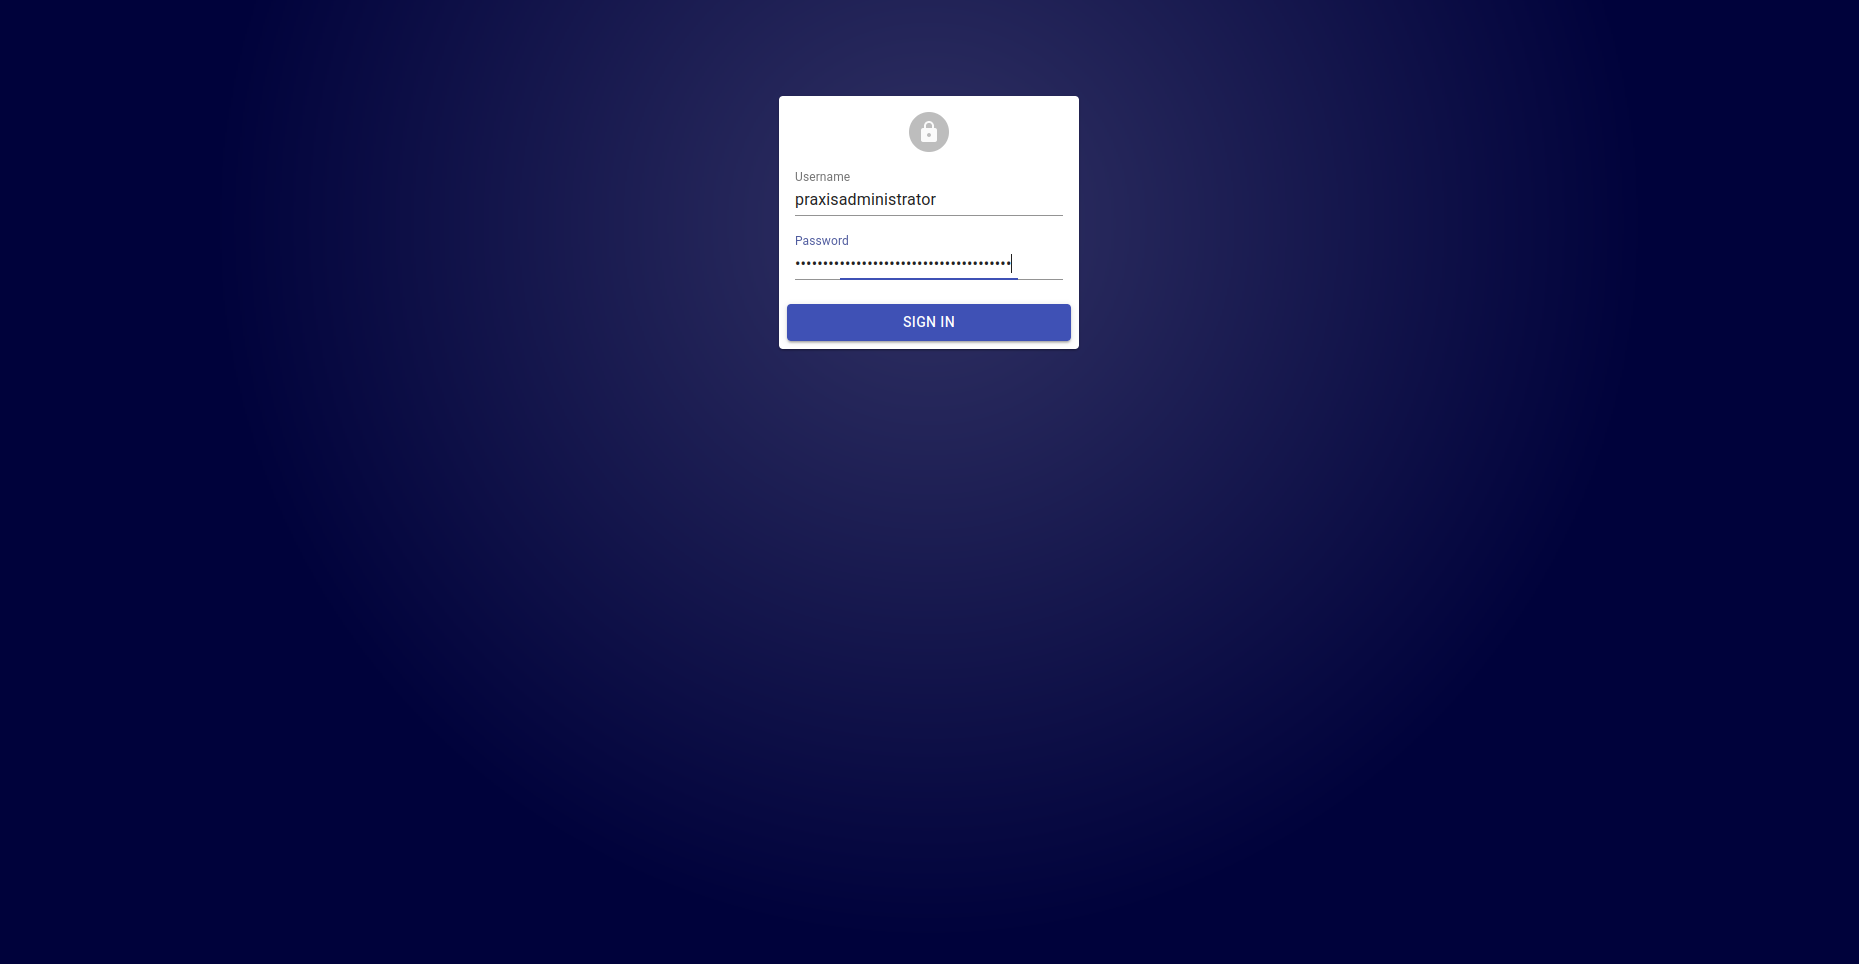
\includegraphics[width=\textwidth]{graphics/screenshots/adminui/login}
        \caption{Login}
    \end{minipage}
    \hfill
    \begin{minipage}[b]{0.4\textwidth}
        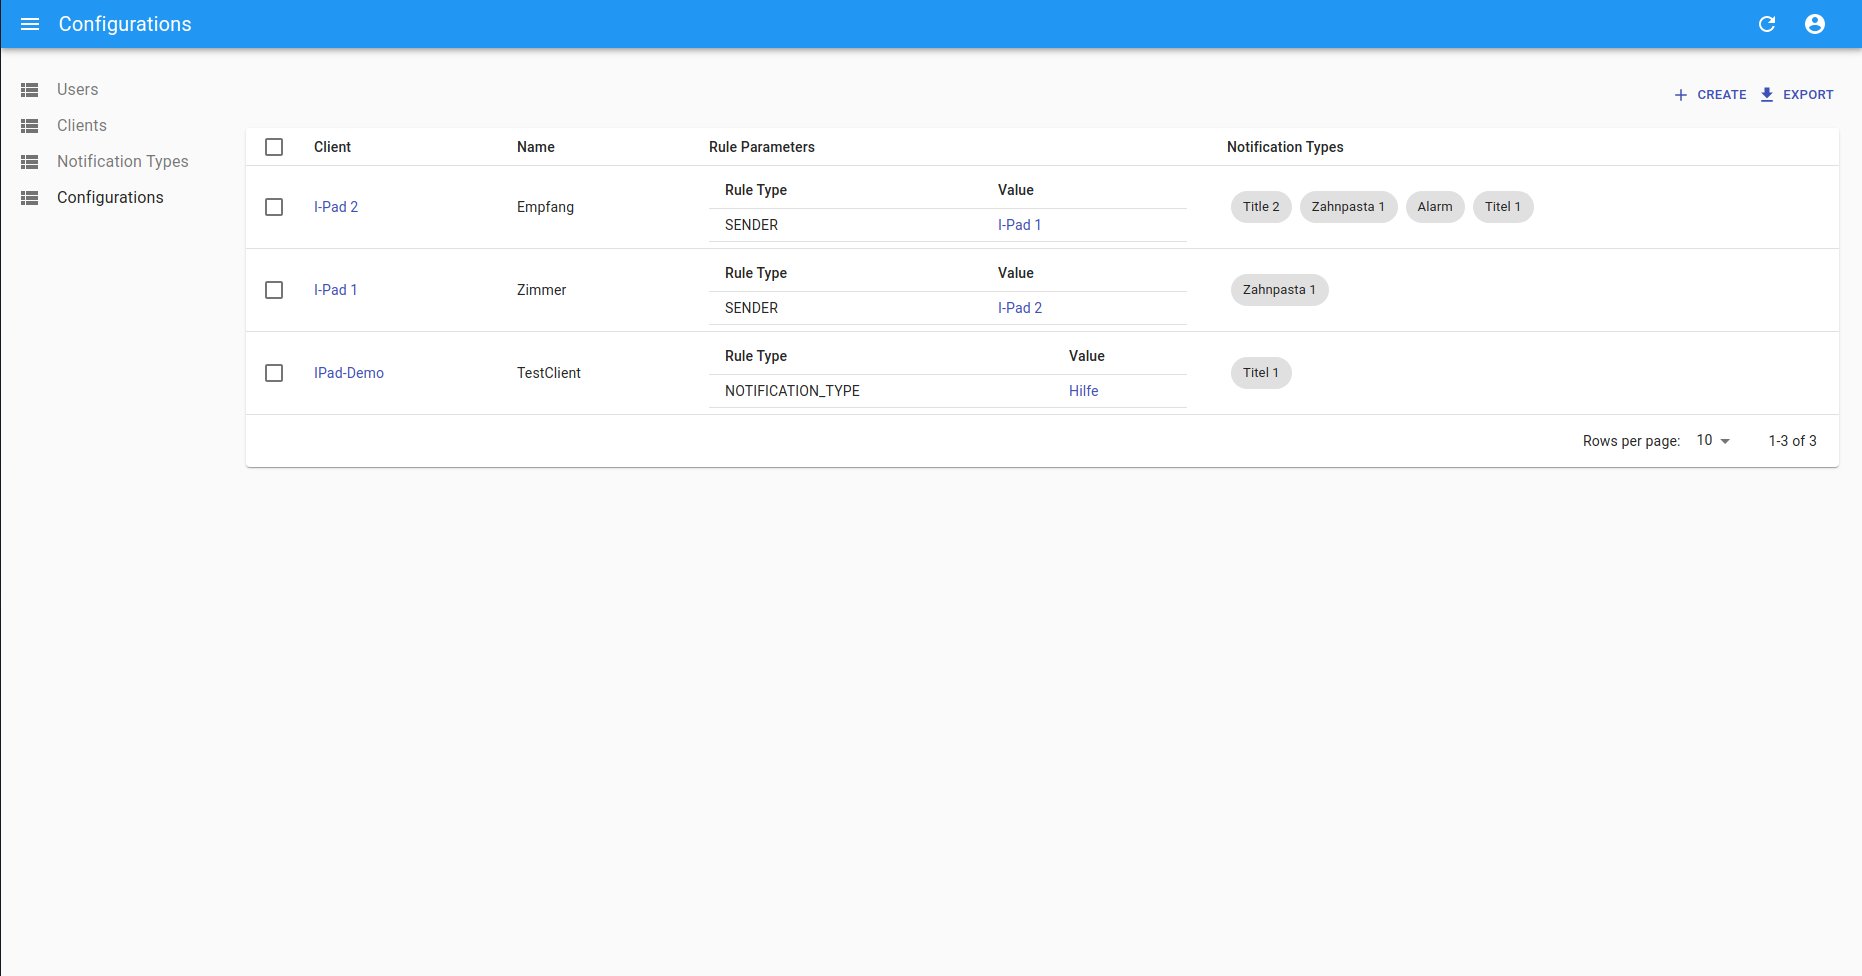
\includegraphics[width=\textwidth]{graphics/screenshots/adminui/configuration-all}
        \caption{Configuration Overview}
    \end{minipage}
    \label{fig:AdminUI-Screens1}
\end{figure}

\begin{figure}[h]
    \centering
    \begin{minipage}[b]{0.4\textwidth}
        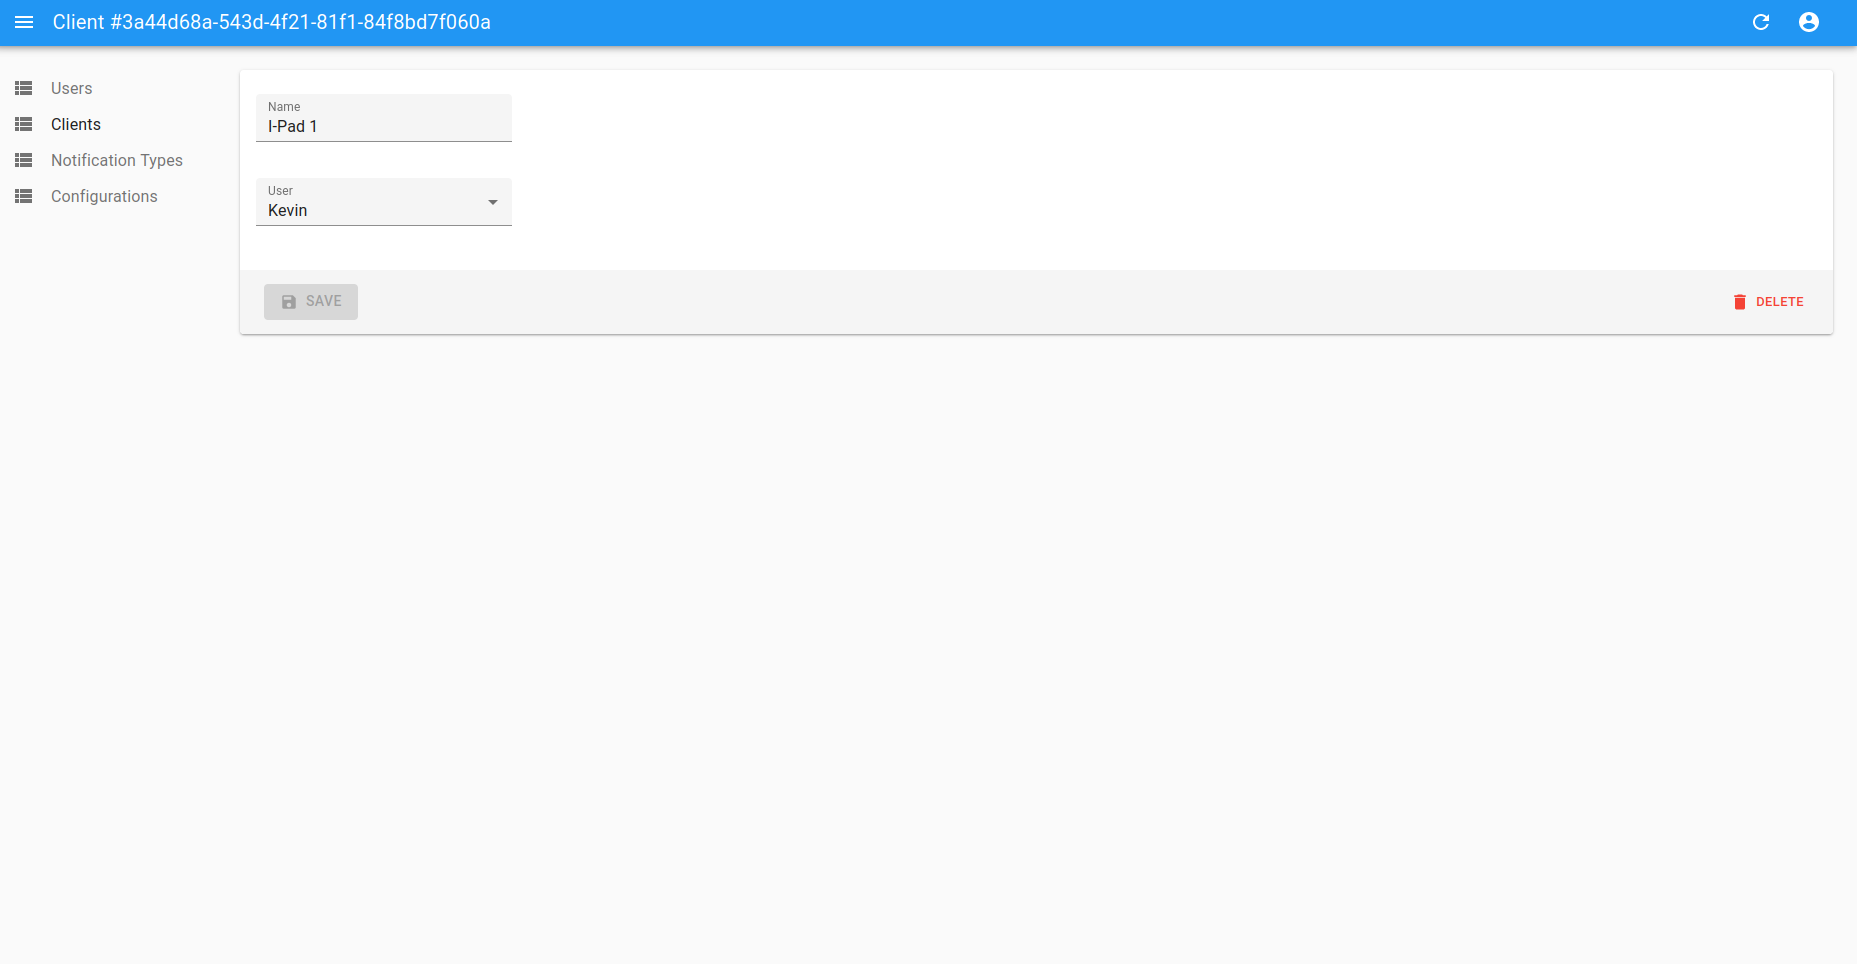
\includegraphics[width=\textwidth]{graphics/screenshots/adminui/configuration}
        \caption{Login}
    \end{minipage}
    \hfill
    \begin{minipage}[b]{0.4\textwidth}
        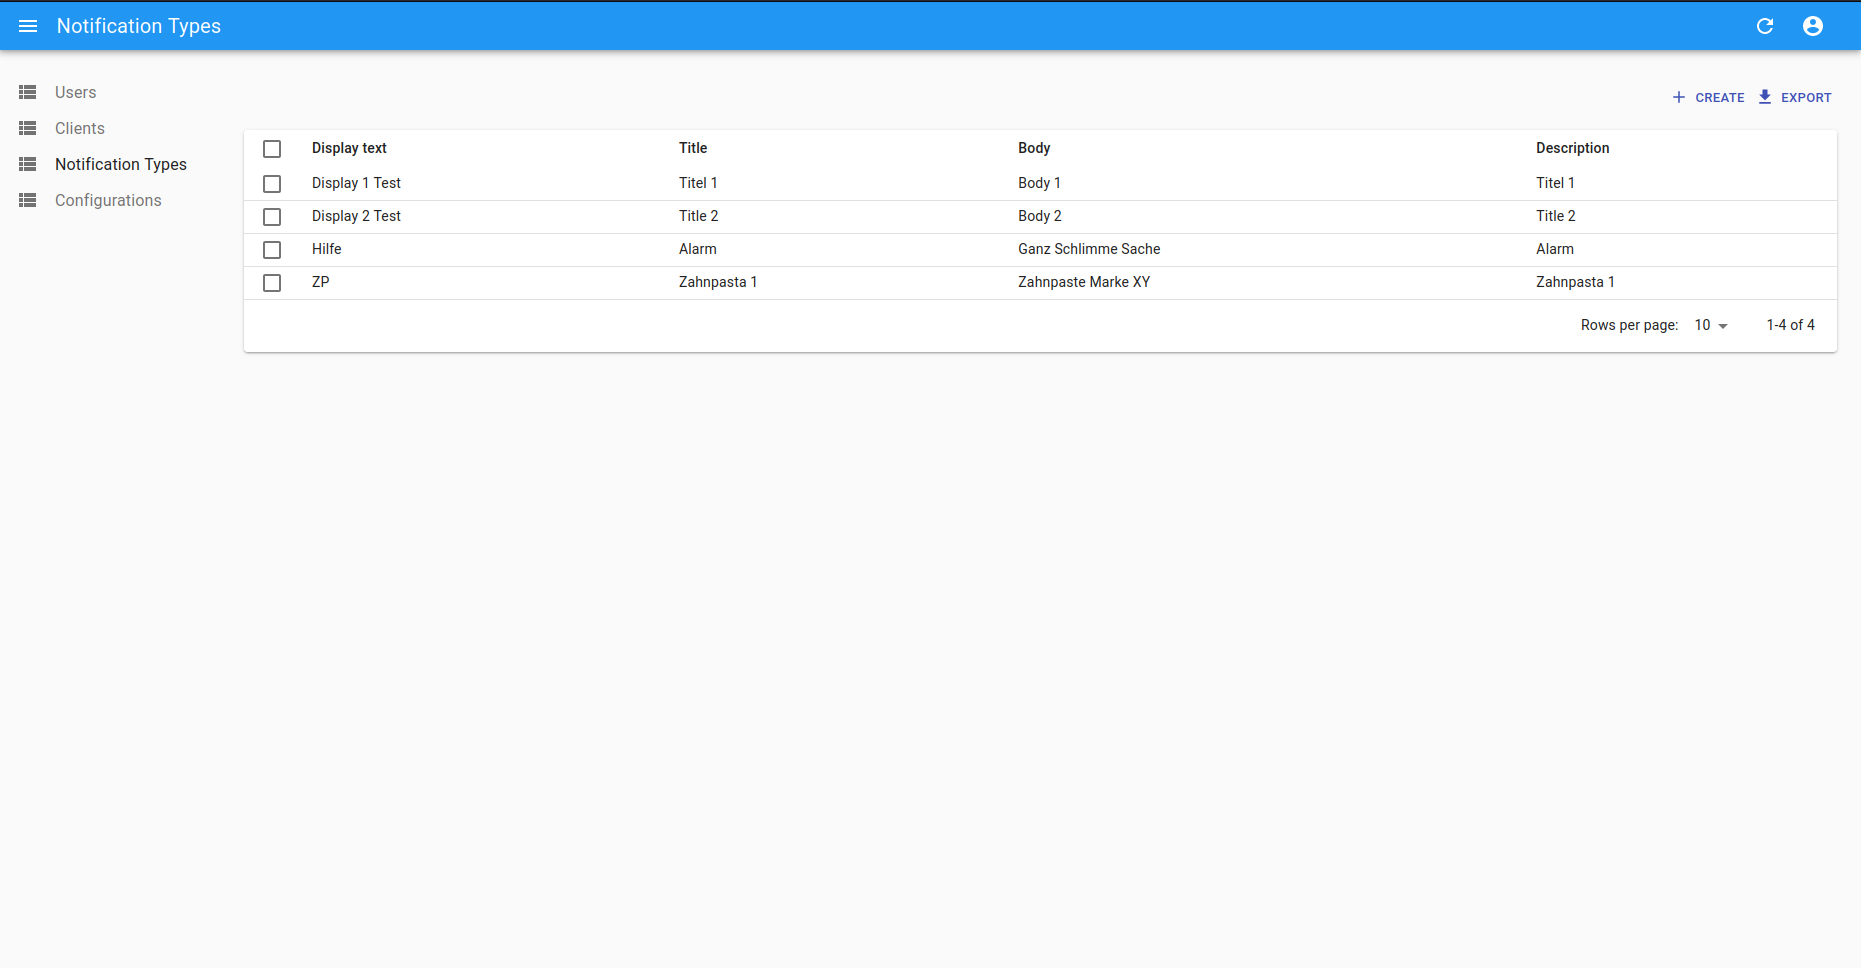
\includegraphics[width=\textwidth]{graphics/screenshots/adminui/notification-type}
        \caption{Configuration Overview}
    \end{minipage}
    \label{fig:AdminUI-Screens2}
\end{figure}




Add some screen shots

\subsection{Tests}

\subsubsection*{Benutzertests}
Wurden mit Daniel Jossen zusannem an der FH gemacht.
Mehr Tests waren wegen Ferienabwesenheiten auf Kundenseite nicht möglich.
Macht nicht so viel sinn mit nur einem Ipad.


\subsubsection*{Benutzertests}
Macht nicht so viel sinn mit nur einem Ipad.

\clearpage
\subsection{Lessons Learned}

Hearusforderungen waren:
\begin{itemize}
    \item Dokumentation fehlt komplett in der Planung
    \item IOS Recherche viel aufwändiger als erwartet.
    \item Nativescript aufwändiger zu gebrauchen als erwartet.
    \item AWS aufsetzen ist alles andere als trivial
    \item Keine Erfahrung mit Mobile Development
    \item Stärkerer Roter Faden von Anfang an hätte geholfen
    \item Mehr testing, viel Mehr Testing.
    \item Refactoring kostet Zeit, kanns aber wert sein.
\end{itemize}

Darus mitgenommen haben wir:
\begin{itemize}
    \item Gute Planung macht sich bezahlt. (Roter Faden, Doku mit einplanen, Standortbestimmung)
    \item Gute Konzepte machen sich bezahlt.
    \item Best Practices gibt es aus einem Grund. (Nativ ist besser)
    \item DevOps ist schwer.
\end{itemize}





